%!TEX root = Nanomat.tex
\ctitle{Å lage tynnfilmer med våtkjemiske metoder}
I dette og neste kapittel skal vi lage tynnfilmer på et substrat. I dette kapittelet ser vi på våtkjemiske metoder (``wet-chemical methods''). Dette betyr i praksis at vi begynner med en løsning eller suspensjon med kildematerialet, og prøver å bruke denne til å dekke substratet.

\cstitle{Surfaktant-tynnfilmer}
\paragraph{Self-assembled monolayers (SAMs)} SAMs er akkurat det de høres ut som - todimensjonale enkeltlag med molekyler på substratet, som organiserer seg selv. SAMS lages ved at man drypper en passende løsning med surfaktanter på et substrat (eller dekker substratet i løsning). Så lener man seg tilbake og venter på at molekylene organiserer seg selv. 

Molekylene det er snakk om i SAMs er surfaktanter. Surfaktantene består av et hydrofilt hode, en alkyl-kjede og en funksjonell gruppe. Disse må oppfylle følgende krav:
\begin{itemize}
	\item Surfaktantens hode må være slik at det foretrekker å kjemisorberes på overflaten av substratet. 
	\item Svake bindinger mellom alkylkjedene sørger for selvorganiseringen.
	\item Hvilken funksjonell gruppe man har på enden av molekylet, avhenger av hvilke egenskaper man vil at filmen skal ha. 
\end{itemize}

Slik dannes SAMs:
\begin{enumerate}
	\item Surfaktanthodene kjemisorberes på substratet. Dette går kjapt, for kjemisorbsjonen er ganske eksoterm hvis vi har vært lure med valg av surfaktant og substrat. Surfaktantene vil prøve å komme seg inn på hvert eneste mulige bindingspunkt på substratet.
	\item Molekylene organiserer seg selv på overflaten gjennom diffusjon, van der Waals-krefter og elektrostatiske krefter. Det har seg slik at den frie energien er minimert når molekylene danner et ganske tettpakket 2D-lag på overflaten av substratet.
\end{enumerate}

Det finnes flere eksempler på materialer vi kan bruke til surfaktanter og til substrater, og bindingen mellom surfaktant og substrat kan være alt mulig:
\begin{itemize}
	\item Alkantioler (\ce{SH-(CH2)_{n}-R}) på en overflate av \ce{Au}, \ce{Ag} eller \ce{Cu}. I dette tilfellet vil det skje en oksidasjonsreaksjon der \ce{S-H}-bindingen brytes, og det dannes \ce{S-M}-bindinger samt hydrogengass. Dialkylsulfider og dialkyl-disulfider funker også -- svovel er generelt glad i disse metallene. I dette tilfellet vil det være en polar kovalent binding mellom svovel og metallet.
	\item Alkoholer og aminer på \ce{Pt}. I dette tilfellet vil det være ionebinding mellom surfaktanten og metallet.
	\item Karboksylsyrer på \ce{AlO} eller \ce{Ag}. Også her blir det ionebinding.
	\item Organosilisium-molekyler der surfaktanthodet er \ce{SiO2}, på et substrat av \ce{Si}. Eller surfaktanthodet kan være \ce{Al2O3} og substratet kan være \ce{Al} eller glass. I dette tilfellet vil det bli en kovalent binding mellom surfaktant og substrat. Hvis den funksjonelle gruppen på surfaktanten er \ce{OH}, kan vi faktisk lage en ny SAM på toppen av det første laget (og slik kan vi fortsette). Men merk at kvaliteten på de øvre lagene ikke vil være like god som kvaliteten på det første laget.
\end{itemize}

\paragraph{Languir-Blodgett-filmer}
Languir-Blodgett-filmer lages ved å dyppe substratet i en væske som har surfaktanter på overflaten, samtidig som man bruker en maskin til å dytte surfaktantene inn på substratet. Det forklares best med en figur:
\begin{figure}[H]
	\bmd\centering
	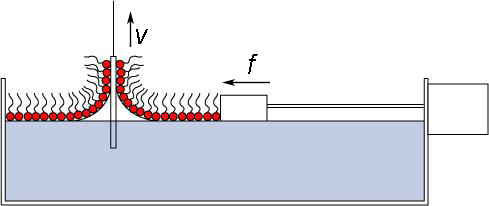
\includegraphics[width=\linewidth]{metodefigs/lb.png}
	\caption{Slik kan man lage Langmuir-Blodgett-filmer.  (av Dbroesch på Wikimedia, lisensiert under CC-BY-SA 3.0)}
	\label{fig:label}
\emd\end{figure}
De viktigste forskjellene mellom SAM og Langmuir-Blodgett-filmer er at I SAMs adsorberes surfaktantene via en kjemisk reaksjon (kjemisorpsjon), mens i Langmuir-Blodgett-filmer adsorberes surfaktantene ved hjelp av de mekaniske kreftene fra maskinen (fysisorpsjon). Dessuten lages ikke Langmuir-Blodgett-filmer ved self-assembly (vi bruker eksterne krefter til å lage filmen).

\cstitle{Chemical solution deposition}
I de tre neste metodene -- dipcoating, spincoating og spraycoating -- begynner vi med en kjemisk løsning, som vi så forsøker å dekke substratet med. Chemical solution deposition er vanlig å bruke med sol-gel-metoder. 

\paragraph{Dipcoating} er veldig enkelt. Dypp substratet i en løsning med det du vil lage tynnfilm av, og trekk den opp. Det viser seg at tykkelsen på filmen er proporsjonal med 
\begin{equation}
	\sqrt{\frac{\eta U_0}{\rho g}},
\end{equation}
 der $\eta$ er viskositeten til løsningen, $U_0$ er hastigheten substratet trekkes opp med, $\rho$ er tettheten til sol-en som dekker substratet, og $g$ er jordakselerasjonen. Merk at filmen blir \emph{tykkere} jo raskere man drar substratet opp, i motsetning til hva man kanskje skulle tro. Jeg har ikke funnet ut hvorfor, men jeg regner med at det er fordi filmen ikke rekker å renne av substratet.
\begin{figure}[H]
\bmd\centering
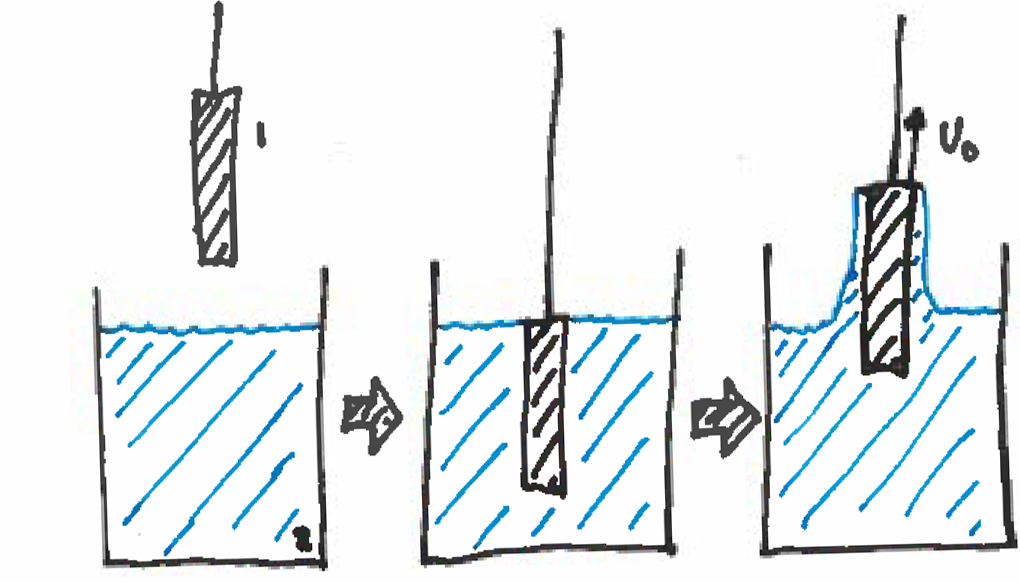
\includegraphics[width=\linewidth]{metodefigs/dipcoat.png}
\caption{Sånn kan man gjøre dip coating. 1: Substrat. 2: Løsning eller suspensjon.}
\emd\end{figure}
Dipcoating kan enkelt parallelliseres (bare dypp en rekke substrater i samme løsning) og kan dermed gjøres på stor skala. Hvis substratet er fleksibelt, kan man videre effektivisere ved å ha substratet på en rull, og kontinuerlig trekke det gjennom løsningen:
\begin{figure}[H]
	\bmd\centering
	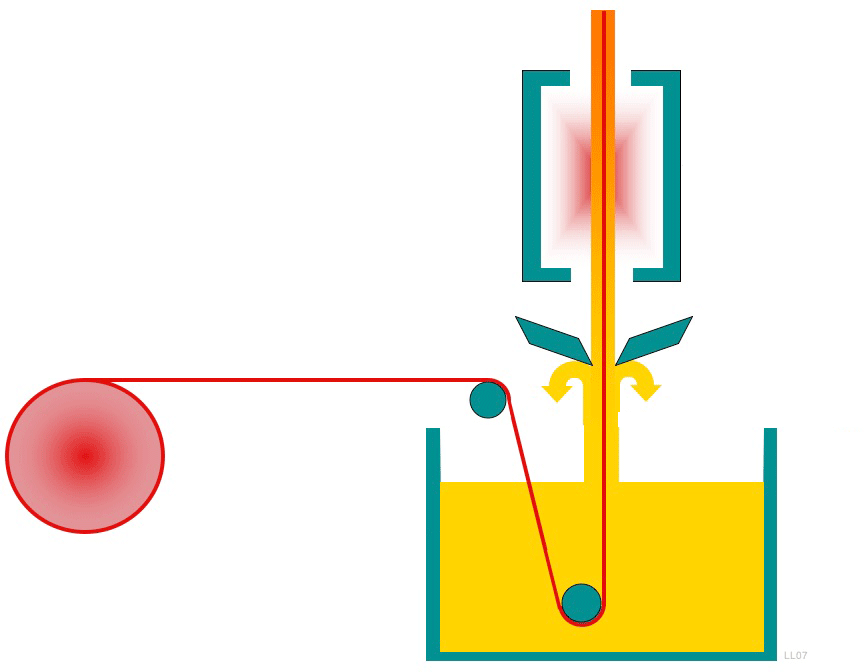
\includegraphics[width=0.8\linewidth]{metodefigs/dipcoatcont.png}
	\caption{Sånn kan man også gjøre dip coating.}
\emd\end{figure}

\paragraph{Spincoating} er også temmelig enkelt: du drypper en passende mengde av løsningen din på substratet. Dette substratet har du festet til en disk, som spinner med høy hastighet for å fordele løsningen jevnt utover substratet. Tykkelsen på filmen blir da proporsjonal med (blant annet)
\begin{equation}
	\frac{\eta}{\omega^2},
\end{equation}
der $\omega$ er vinkelfrekvensen til disken. Andre faktorer som påvirker tykkelsen og mikrostrukturen til filmen er måten løsningen dekker substratet på, tiden man bruker på å spinne, mengden løsning man putter på, pH, antall lag man putter på, og tørking/oppvarming etter at man har spunnet disken. Avhengig av disse parametrene kan man få defekter som luftbobler, ujevn filmtykkelse og spiralmønstre i filmen.
\begin{figure}[H]
\bmd\centering
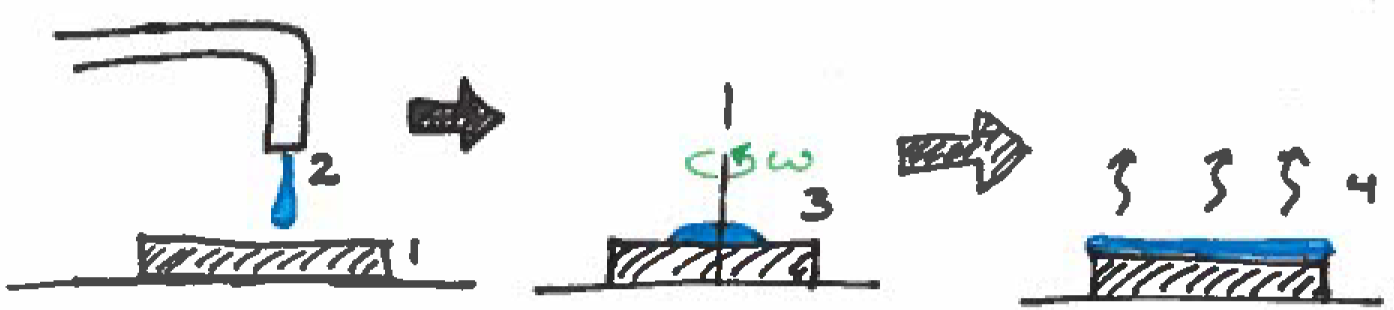
\includegraphics[width=\linewidth]{metodefigs/spincoat.png}
\caption{Sånn kan man gjøre spin coating. 1: Substrat. 2: Løsning dryppes på substratet. 3: Rotasjon sprer løsningen som en jevn film gjennom sentrifugalkrefter. 4: Løsemiddelet fordamper.}
\emd\end{figure}
Spincoating er ikke like enkelt å oppskalere som dipcoating, for du må jo feste og spinne hver enkelt disk hver for seg.

\paragraph{Problemer med dip- og spincoating} Hovedproblemet med de to ovennevnte metodene er at det fort kan dannes sprekker i filmen. Dette kan skje hvis
\begin{enumerate}
	\item gel-en begynner å krympe for mye når løsemiddelet fordamper
	\item det begynner å bli polymerisering og krysslinking i gel-matrisen
	\item kapillærkrefter trekker og strekker på gel-en (også på grunn av fordamping av løsemiddelet, se kapittelet om sol-gel)
	\item substratet og filmen har forskjellige varmeutvidelseskoeffisienter
\end{enumerate}
Vi kan unngå sprekkdannelse ved å
\begin{enumerate}
	\item la filmen ha større bruddseighet (duh)
	\item la filmen være mer elastisk (lavere Youngs modulus)
	\item redusere mengden løsemiddel i løsningen når den begynner å stivne
	\item redusere tykkelsen på filmen
\end{enumerate}

\paragraph{Spray coating} Du har en gass-strøm som trekker med seg kjemiske forløpere til filmen i en spray.
\begin{figure}[H]
\bmd\centering
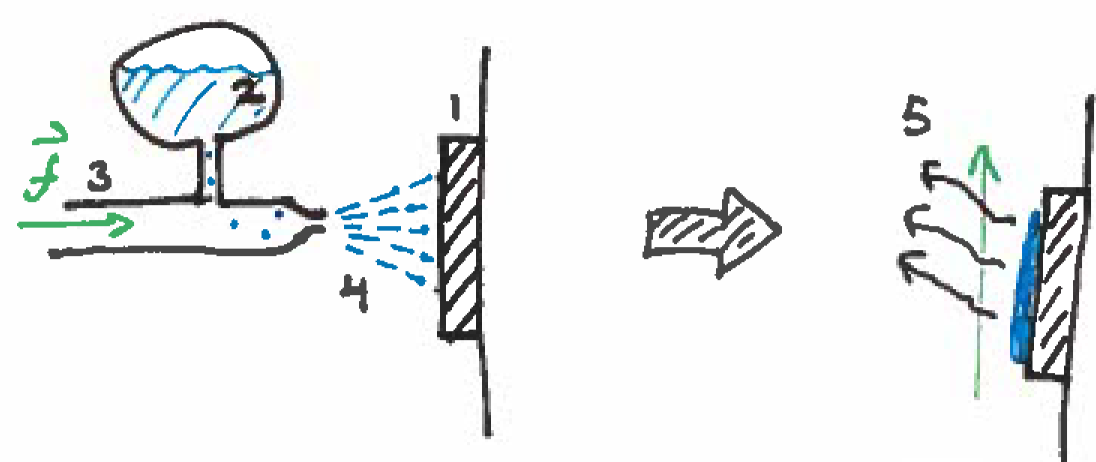
\includegraphics[width=0.7\linewidth]{metodefigs/spraycoat.png}
\caption{Sånn kan man gjøre spray coating. 1: Substrat. 2: Løsning. 3/4: Løsningen blåses mot substratet i form av en spray som treffer substratet. 5: Løsemiddel samt dråper og pulver av løsningen blåses vekk.}
\emd\end{figure}
Dette er veldig enkelt, kan gjøres ved lav temperatur, er lett å skalere opp og automatisere, og kan gjøres med en rekke forskjellige materialer på en rekke forskjellige substrater. Det kan brukes til å lage dopede eller graderte filmer, eller filmer som består av flere lag.

Dessverre er metoden sensitiv for støv, det er ikke lett å få en film med uniform tykkelse, og det er nødvendig med varmebehandling til slutt for å få filmen tett og sterk nok.

\paragraph{Bruksområder for dip- og spin coating} Filmene vi lager med de to ovennevnte metodene kan brukes til å lage beskyttende belegg (mot korrosjon og oksidasjon), optiske belegg (for å forbedre speil og linser), fotosensitive resister i litografi, og ferromagnetiske belegg i datamaskinminne. Vi kan også lage belegg som endrer egenskapene til overflater (for eksempel ved å gjøre dem glattere eller vannavstøtende), eller bruke dem til å lage systemer for drug-delivery.

\paragraph{Elektrokjemisk deponering} er å lage en reversert galvanisk celle der katoden er substratet. Kationer i løsningen går mot substratet og inngår i en reduksjonsreaksjon der. 
\begin{figure}[H]
\bmd\centering
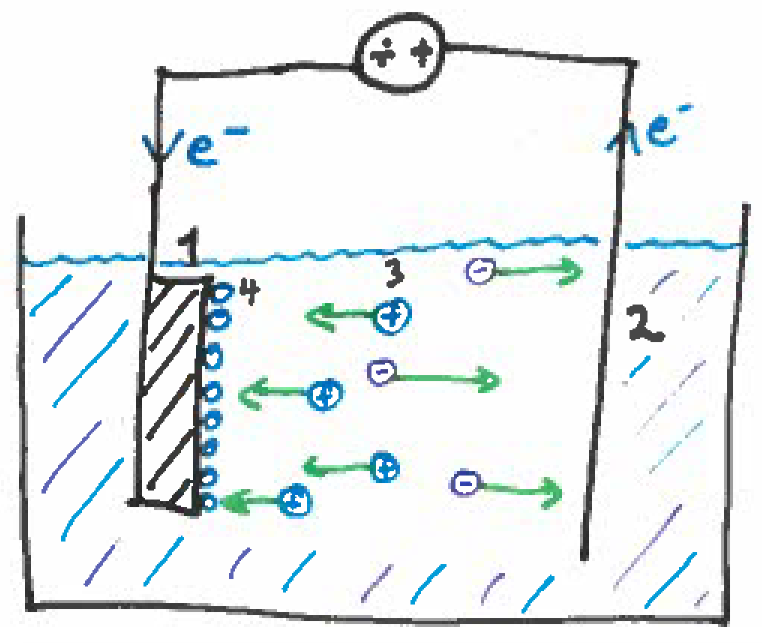
\includegraphics[width=0.6\linewidth]{metodefigs/elkjemdep.png}
\caption{Sånn kan man gjøre elektrokjemisk deponering. 1: Substrat (også katoden). 2: Anode. 3: Kationene i løsningen går mot katoden. 4: Kationene reduseres på substratet og danner en (elektrisk ledende) film.}
\emd\end{figure}
Metoden er fin for å lage tynnfilmer av metaller, for det er i hovedsak ledningsevnen til substratet (og den deponerte filmen) som bestemmer prosessforløpet. Siden substratet skal være en elektrode, må det være elektrisk ledende. Og hvis filmen ikke er ledende, vil deponeringen stoppe når det første laget har dannet seg på elektroden. Så: jo lavere konduktiviteten til filmen er, jo mindre blir den maksimale tykkelsen til filmen. Filmen blir også mer ujevn hvis materialet er en dårlig leder.

Hvis reduksjonspotensialet til materialet man skal deponere er lavere enn reduksjonspotensialet til vann, altså hvis det er et veldig edelt metall, kan man ikke bruke vann. Dette fordi du ender opp med å hydrolysere vannet i stedet (samme problem som i Cushing, da vi skulle bruke reduksjon av metall til å lage nanopartikler). I så fall må man bruke ikke-vandige løsemidler eller en saltsmelte.

\paragraph{Elektroforetisk deponering} er elektrokjemisk deponering der du bruker en suspensjon av kolloidale partikler i stedet for en løsning. Disse kolloidale partiklene må være elektrisk ladet i suspensjonen, men de trenger ikke å være elektrisk ledende. Ellers gjelder de samme prinsippene som for elektrokjemisk deponering.

I dette tilfellet slipper vi som regel problemene med egenelektrolyse av vann, for det er ikke en reduksjonsreaksjon som forårsaker filmdannelse -- det er det elektriske feltet mellom elektrodene som trekker partiklene mot den ene elektroden.

En ulempe med elektroforetisk deponering er at du ikke kan lage veldig tynne filmer med denne metoden - filmens tykkelse er begrenset av størrelsen til partiklene.
